\documentclass[vipdfmx,a4paper,11pt]{jsarticle}
\usepackage{hyperref} % ハイパーリンク差し込み用
\usepackage{pxjahyper} % 目次の文字化け対策

\usepackage[dvipdfmx]{graphicx,xcolor}% ドライバ指定のため

%オートマトン
\usepackage{tikz}
\usetikzlibrary{automata,positioning}
\usetikzlibrary{calc}
\usetikzlibrary{decorations.pathreplacing}
\usetikzlibrary{matrix,backgrounds,fit,positioning}

% 数式
\usepackage{amsmath,amsfonts}
\usepackage{amssymb}
\usepackage{bm}
\usepackage{braket}
\usepackage{multicol}

% 画像
\usepackage[dvipdfmx]{graphicx}

% SI単位
\usepackage{siunitx}

%プログラムリスト用
\usepackage{listings,jvlisting}
\lstset{
basicstyle={\ttfamily},
identifierstyle={\small},
commentstyle={\smallitshape},
keywordstyle={\small\bfseries},
ndkeywordstyle={\small},
stringstyle={\small\ttfamily},
frame={tb},
breaklines=true,
columns=[l]{fullflexible},
numbers=left,
xrightmargin=0zw,
xleftmargin=3zw,
numberstyle={\scriptsize},
stepnumber=1,
numbersep=1zw,
lineskip=-0.5ex
}

\usepackage{tcolorbox}
\newtcbox{\code}[1][]{
  colback=gray!10!white,
  colframe=gray!20!white,
  boxrule=1pt,
  left=0mm,right=0mm,top=0mm,bottom=0mm,
  box align=base,
  nobeforeafter,
  fontupper=\ttfamily
}

\renewcommand{\thesubsection}{\arabic{section}-\arabic{subsection}}
\renewcommand{\thesubsubsection}{\arabic{section}-\arabic{subsection}.\arabic{subsubsection}}
\makeatletter
  \renewcommand{\theequation}{\arabic{subsection}.\arabic{equation}}
  \@addtoreset{equation}{subsection}
\makeatother
\makeatletter
% sectionの下マージンを小さく
\renewcommand{\section}{%
  \@startsection{section}{1}{\z@}%
  {0.4\Cvs}{0.1\Cvs}%
  {\normalfont\large\headfont\raggedright}}
\renewcommand{\subsection}{%
  \@startsection{subsection}{1}{\z@}%
  {0.4\Cvs}{0.1\Cvs}%
  {\normalfont\large\headfont\raggedright}}
\renewcommand{\subsubsection}{%
  \@startsection{subsubsection}{1}{\z@}%
  {0.4\Cvs}{0.1\Cvs}%
  {\normalfont\large\headfont\raggedright}}
\makeatother

\begin{document}

\title{MMCSS tutorial(jp)}
\author{Takanori Saiki}
\date{最終更新日 : \today}
\maketitle

\newpage

\section{はじめに}
MMCSS(Multicellular Molecular Communication System Simulator)は多細胞分子通信系のシミュレーションを実施する汎用シミュレータです。
シミュレーションにおいて基盤となるプログラムは用意されているので、ユーザはパラメータを変更することで、
あるいは独自に拡張をおこなうことで自身の考えたシミュレーションモデルを簡単に実装することができます。

\section{導入}
ここでは、MMCSSを導入するための手順を説明します。使用環境はMac OSかLinuxを想定していますが、
いくつかのツールを揃えることでWindowsでも実行可能になります。

\subsection{ダウンロード}
GitHubのMMCSSのページ(\href{https://github.com/saikiRA1011/CellNetworkShapeSimulation}{https://github.com/saikiRA1011/CellNetworkShapeSimulation})
からソフトウェアをダウンロードします。ダウンロード先はどこでも良いですが、シミュレーションの実行後に画像ファイルや
動画ファイルが作成されるため容量の余裕があるドライブに配置しましょう。

\subsection{セッティング}
MMCSSではいくつかの外部ツールをシミュレーションの作成、実行に用いています。以下はそのツールとバージョンの一例です。
\begin{itemize}
  \item gcc 11.3.0 (C++11が使用できるバージョン)
  \item Python 3.9.12
  \item pip 22.1.2
  \item make 3.81
  \item yaml-cpp 0.8
\end{itemize}

Makefileではgcc-14を使用していますが、インストールされているgccのバージョンに合わせて変更してください。
またOpenMPを使用しているため、他のコンパイラは使用にあたって注意が必要です。

Pythonで用いるライブラリは以下のコマンドから一括でインストールできます。

\begin{lstlisting}
  pip install -r requirements.txt
\end{lstlisting}

\section{実行}
ここではシミュレーションの実行方法を説明します。MMCSSではmakeを用いてビルド・シミュレーション実行・動画ファイルの生成を実行できるようにしています。

シミュレータをビルドする際には単に、\code{make}を実行してください。実行ファイルとしてSimMainが生成されます。
また、シミュレーションを実行する際には\code{make run}を実行してください。シミュレーション結果はresultディレクトリに、ステップごとに
テキストファイルとして出力されます。次に、シミュレーション結果から動画ファイルを生成する際には\code{make convert}を実行してください。
最終生成物のout.mp4はvideoディレクトリに、中間生成物の各ステップごとの画像はimageディレクトリに出力されます。最後に、
生成した動画を確認したい時は\code{make open}を実行してください。

% シミュレーションの設定を変更した際は、そのまま\code{make}すると修正前のオブジェクトファイルを参照してしまうことがあるので、
% 事前に\code{make clean}を実行してすべてのオブジェクトファイルを削除してください。

また、これらの一連の処理は\code{make all}でまとめて実行可能です。図\ref{fig:appMake}に一連の流れを示します。

\begin{figure}[tbp]
  \centering
  \fbox{
    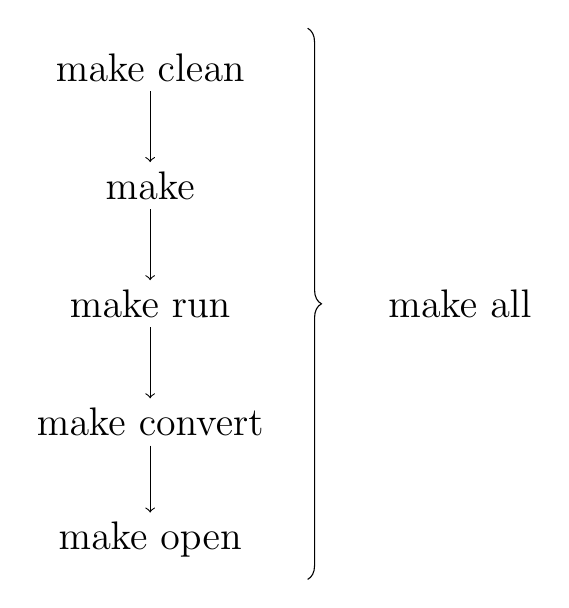
\begin{tikzpicture}[node distance=1.5cm]
      \node[](clean){\code{\Large{make clean}}};
      \node[below of=clean](make){\code{\Large{make}}};
      \node[below of=make](run){\code{\Large{make run}}};
      \node[below of=run](convert){\code{\Large{make convert}}};
      \node[below of=convert](open){\code{\Large{make open}}};
      \node[right of=run, right=1.4cm](all){\code{\Large{make all}}};
      \draw[->] (clean)--(make);
      \draw[->] (make)--(run);
      \draw[->] (run)--(convert);
      \draw[->] (convert)--(open);
      \draw[decorate,decoration={brace,amplitude=5}, right of=run, right=1.5cm]
      ($(clean)+(2.0cm,0.5cm)$)--($(open)+(2.0cm,-0.5cm)$);
    \end{tikzpicture}
  }
  \caption{make コマンドによる一連の流れ}
  \label{fig:appMake}
\end{figure}

\section{シミュレーションの自作}
ユーザは自身でプログラムを書くことで(あるいはパラメータを変更することで)、シミュレーションを自作することができます。
また、ファイルの内容をデフォルトに戻したい場合は、\ref{make}で解説している\code{make reset}を実行することで初期化できます。
ここでは、ユーザが編集するファイルごとにシミュレーションの自作に必要な知識を説明します。

\subsection{config.yml, SimulationSettings.hpp(.cpp)}
config.ymlとSimulationSettings.hpp(.cpp)にはシミュレーションに必要となるパラメータを定義します。例えば、シミュレーションのステップ数や、
Cell(バイオナノマシン)の個数、シミュレーションのstepあたりの単位時間です。
それぞれのパラメータの説明は当該ファイルにコメントとして記述されているので、それらを参考にしてください。

また、必要であればパラメータを増やすことも可能です。
自身で必要だと思ったシミュレーションのパラメータをSimulationSettings.hppに追加し、SimulationSettings.cppにyamlファイルからの読み取り用コードをtryブロック内に追記してください。
またこれらパラメータはstatic変数として定義されるので、必ずSimulationSettings.cpp末尾で初期化してください。

パラメータを設定したい場合は、config.yamlにkeyと値を記述してください。また、自身で定義したパラメータがある場合は、このファイルにも追記することを忘れないでください。

\text{\color{red} デフォルトで用意されているパラメータを削除することはできません。}

\subsection{UserSimulation.hpp(.cpp)}
UserSimulation.hpp(.cpp)にはシミュレーションのモデルや初期条件(Cellの分布など)を定義することができます。
現在定義可能な関数は、Cellの初期化(initCells)、ステップ実行前処理(stepPreprocess)、細胞間に働く力学モデル(calcCellCellForce)、ステップ実行後処理(stepEndProcess)に加え、細胞間相互作用の計算(calcCellCellForce)のみです。

シミュレーションで用いる細胞の種類や分子の種類などもここで定義します。

このファイルもSimulationSettings.hppと同様、ユーザが独自に変数・関数を定義することができるます。実装したいモデルに合わせて
関数を追加・変更してください。

\subsection{UserCell.hpp(.cpp)}
UserCell.hpp(.cpp)には細胞の挙動を定義することができます。

例えば、細胞の死滅タイミングや、分裂タイミング、代謝によるエネルギーや保有分子濃度の変化等を実装することができます。

細胞の増減を実装するにあたりユーザが最も苦労することは現存する細胞のリストをどのように管理するかです。
MMCSSではこの面倒な管理をCell.hpp(.cpp)内で実装しているため、ユーザは細胞がいつ・どのような状況で増減するかのみを実装することで
シチュエーションを再現できます。

\subsection{UserMoleculeSpace.hpp(.cpp)}
UserMoleculeSpace.hpp(.cpp)にはシミュレーションで扱いたい分子の系を定義することができます。

親クラスであるMoleculeSpaceにいくつかの境界条件(ノイマン条件や、ディリクレ条件、PBC)が実装されているため、
これらの境界条件を用いる際はユーザが処理を追加する必要はありません。

またMoleculeSpaceはCellと相互的に作用させることができるように、お互いに参照を持つように実装してあります。
この機能はUserMoleculeSpaceとUserCellにも引き継がれているため、細胞と分子の複雑な相互作用をシミュレーションする際でも、ユーザは
面倒なクラス間の参照関係を実装する必要はありません。

\newpage
\section{付録A}
\subsection{シミュレーションの結果のファイル}
シミュレーションを実行するとresultディレクトリに cells\_step番号 のファイル名で複数のテキストファイルが出力されます。
これがシミュレーションの結果を出力したものです。

テキストファイルの中身はタブ文字区切りで、以下の形式でシミュレーション結果が記されています。

\begin{lstlisting}
  ヘッダ行
  ID typeID X Y Z Vx Vy Vz R N_contact Contact_ID_1 Contact_ID_2 ...
\end{lstlisting}

それぞれのデータの説明は以下の通りです。

\begin{itemize}
  \item ID : Cellの識別子。唯一無二のものが割り当てられる
  \item typeID : Cellの種類の識別子。種類ごとに異なる動作を定義できる
  \item X : CellのX座標の位置
  \item Y : CellのY座標の位置
  \item Z : CellのZ座標の位置
  \item Vx : CellのX方向の速度
  \item Vy : CellのY方向の速度
  \item Vz : CellのZ方向の速度
  \item R : Cellの半径
  \item N\_contact : 接触しているCellの数
  \item Contact\_ID : 接触しているCellのID
\end{itemize}

\subsection{makeコマンド}\label{make}
MMCSSではシミュレーションの実行から結果の確認に関わるmakeコマンド以外にも、いくつかのコマンドを用意しています。
以下はそれらの解説です。

\begin{itemize}
  \item \code{make} : プログラムをビルドする。
  \item \code{make run} : シミュレーションを実行する。
  \item \code{make convert} : シミュレーション結果を動画ファイルに変換する。
  \item \code{make open} : シミュレーション結果の動画ファイルを確認する。
  \item \code{make clean} : オブジェクトファイルをすべて削除する。
  \item \code{make all} : オブジェクトファイルをすべて削除してから、シミュレーションのビルド、実行、動画の生成、確認を一通りおこなう。
  \item \code{make reset} : シミュレーションのユーザ設定ファイルをデフォルトに戻す。
  \item \code{make data-cleanup} : シミュレーションの生成物(テキスト、画像、動画)をすべて削除する。
  \item \code{make data-archive} : 現在保存されてあるシミュレーション結果をzipアーカイブする。
  \item \code{make archive-restore date=YYYYMMDD\_HHmm} : アーカイブファイルの日時を指定することで、アーカイブの内容を復元する。
  \item \code{make archive-cleanup} : すべてのアーカイブファイルを削除する。
  \item \code{make help} : Makefileに登録されているコマンドの使用方法と説明を表示する。
\end{itemize}

\section{付録B : サンプルコード}
\subsubsection{回転モデル}
\begin{lstlisting}[caption=calcCellCellForce()]
  auto aroundCells            = cellList.aroundCellList(c);
  Vec3 force                  = Vec3::zero();
  const Vec3 center           = Vec3(0, 0, 0);
  const Vec3 diff_from_center = c->getPosition() - center;
  Vec3 force_cont             = Vec3::zero();

  constexpr double COEFFICIENT   = 1.0;
  constexpr double REPUlSION_C   = 0.20;
  constexpr double REPULSION_LEN = 15;
  constexpr double BONDING_LEN   = 5;

  force += -diff_from_center.normalize().timesScalar(COEFFICIENT);

  for (auto i : aroundCells) {
      auto cell = cells[i];

      if (c->id == cell->id)
          continue;

      const Vec3 diff   = c->getPosition() - cell->getPosition();
      const double dist = diff.length();

      if (dist < REPULSION_LEN) {
          force += diff.timesScalar(1.0 / dist).timesScalar(REPUlSION_C).timesScalar((REPULSION_LEN - dist) / REPULSION_LEN);
      }

      const Vec3 v = cell->getVelocity();
      if (dist < BONDING_LEN) {
          force_cont += v;
      }
  }

  force += force_cont.normalize().timesScalar(0.2);
  force = force.timesScalar(SimulationSettings::DELTA_TIME);

  return force;
\end{lstlisting}

\subsubsection{成長モデル}
\begin{lstlisting}[caption=class UserCell]
  // add member variables
  private:
  std::vector<std::vector<bool>> bondMatrix;
    const double dMax   = 150.0;
    const double dMin   = 80.0;
    const double dCont  = 20.0;
    const double lambda = 20.0;
\end{lstlisting}

\begin{lstlisting}[caption=UserSimulation()]
  UserSimulation::UserSimulation(/* args */)
  {
    bondMatrix.resize(SimulationSettings::CELL_NUM, std::vector<bool>(SimulationSettings::CELL_NUM, false));
  }
\end{lstlisting}

\begin{lstlisting}[caption=initCells()]
  void UserSimulation::initCells() noexcept
  {
    std::uniform_real_distribution<double> rand_r(0, 150);
    std::uniform_real_distribution<double> rand_theta(0, 2 * M_PI);
    for (int i = 0; i < SimulationSettings::CELL_NUM; i++) {
        double r     = rand_r(rand_gen);
        double theta = rand_theta(rand_gen);

        double x = r * std::cos(theta);
        double y = r * std::sin(theta);

        UserCell c(CellType::WORKER, x, y, 10);
        cells.push_back(std::make_shared<UserCell>(c));
    }
  }
\end{lstlisting}

\begin{lstlisting}[caption=stepPreprocess()]
  void UserSimulation::stepPreprocess() noexcept
  {
      int32_t preCellCount = cells.size();
  
      for (int i = 0; i < preCellCount; i++) {
          cells[i]->initForce();
      }
  
      for (int i = 0; i < preCellCount; i++) {
          cells[i]->clearAdhereCells();
          for (int j = 0; j < preCellCount; j++) {
              if (i == j) {
                  continue;
              }
  
              const Vec3 diff   = cells[i]->getPosition() - cells[j]->getPosition();
              const double dist = diff.length();
              if (dist <= dCont) {
                  bondMatrix[i][j] = true;
              }
  
              if (bondMatrix[i][j] && dist >= dMax) {
                  bondMatrix[i][j] = false;
              }
  
              if (bondMatrix[i][j]) {
                  cells[i]->adhere(*cells[j]);
              }
          }
      }
  }
\end{lstlisting}

\begin{lstlisting}[caption=calcCellCellForce()]
  Vec3 UserSimulation::calcCellCellForce(std::shared_ptr<UserCell> c) const noexcept
  {
      Vec3 force = Vec3::zero();
  
      for (auto cell : cells) {
          if (c->id == cell->id)
              continue;
  
          const Vec3 diff   = c->getPosition() - cell->getPosition();
          const double dist = diff.length();
  
          if (bondMatrix[c->id][cell->id]) {
              if (c->adhereCells.size() <= 3) {
                  force += diff.normalize().timesScalar((dMax - dist) / dMax).timesScalar(2.0);
              } else {
                  force += -diff.normalize().timesScalar(std::max(0.0, (dist - dMin) / (dMax - dMin))).timesScalar(2.0);
              }
          }
  
          force += -diff.normalize().timesScalar(std::exp(-dist / lambda)).timesScalar(0.05);
  
          if (dist < dCont) {
              force += diff.normalize().timesScalar((dCont - dist) / dCont).timesScalar(10.0);
          }
      }
  
      force = force.timesScalar(SimulationSettings::DELTA_TIME);
  
      return force;
  }
\end{lstlisting}

\end{document}